%=======================================================================

% Template modified by Manjil P. Saikia on the basis of the one by Avner Magen %
%=======================================================================
\def\lectureNr{0}   %enter number!
\def\lecture{How to write the lecture notes} %select and enter title
\def\scribe{Manjil P. Saikia}           %enter your name


%%%%%%%%%%%%%%%%%%%%%%%%%%%%%%%%%%%%%%%%%%%%
% DON'T CHANGE ANYTHING IN THE NEXT LINES
\def\solitude{1} %KEEP THIS WAY!!!
\ifnum\solitude=1
 \documentclass[10pt]{article}
 \usepackage[nousetoc,nohylinks]{template}
\fi
%%%%%%%%%%%%%%%%%%%%%%%%%%%%%%%%%%%%%%%%%%%%



%%%%%%%%%%%%%%%%%%%%%%%%%%%%%%%%%%%%%%%%%%%%%%%%%%%%%%%%%%%%%%%%
% YOU MAY ADD ADDITIONAL (PRIVATE) MACROS HERE,
% BUT DO START EACH WITH YOUR INITIALS.
% FOR EXAMPLE, YOUR NAMES IS Anil Kapoor
% THEN START EACH MACRO WITH AK.
% EXAMPLE:
%\newcommand{\AKnorm}[2]{\|#1\|_{_#2}}
%

%%%%%%%%%%%%%%%%%%%%%%%%%%%%%%%%%%%%%%%%%%%%%%%%%%%%%%%%%%%%%%%%

\BEGINDOC
\makeheader
%%%%%%%%%%%%%%%%%%%%%%%%%%%%%%%%%%%%%%%%%%%%%%%%%%%%%%%%%%%%%%%%%%%%%%%%%
% BEGIN BODY of Document

\begin{summary} We explain how to write the lecture notes for the
course ``Optimization Techniques''.
\textbf{You should submit the notes to me by email
(\texttt{manjil@iiitmanipur.ac.in}) not later than Saturday of the week following the lectures you are transcribing.}
\end{summary}

\section{What should the notes contain?}

The notes should contain at least all the material presented in
the lecture. You don't have to follow the exact way in which the
material was presented. Important points:

\begin{enumerate}

\item The notes should contain full proofs even if in
class I skipped some parts or only provided proof
sketches.

\item The lecture notes should contain not only theorems and proofs but
also high level comments and explanations as and when required.

\item The lecture notes should also contain all the exercises and examples given in the lectures and relevant problem sheets.

\item If you have any problems with understanding part of the
material in class \textbf{don't hesitate to ask me for explanations and clarifications}.
\end{enumerate}

\section{Basic steps in writing the notes}

I assume you know how to use \LaTeX. If not, see the next section.

\begin{enumerate}

\item Download the files \texttt{template.tex} ,
\texttt{template.sty} and \texttt{template.bib} from the course's
homepage
(\url{https://manjilsaikia.in/teaching/IIIT/ma305})
and put them in the same directory.

\item Rename the files \texttt{template.tex} and
\texttt{template.bib} to \texttt{week$x$.tex} and
\texttt{week$x$.bib}, where $x$  is your week number.

\item Open the file \texttt{week$x$.tex} and do the following:
\begin{itemize}
\item Change the definitions at the top of the files to your
name(s), the week number, and the title of the lecture.

\item Delete all the lines between the lines marked by
\begin{verbatim}
%%%%%%%%%%%%%%%%%%%%%%%%%%%%%%%%%%%%%%%%%%%%%
% BEGIN BODY of Document
\end{verbatim}

and the lines marked by
\begin{verbatim}
% END BODY of document
%%%%%%%%%%%%%%%%%%%%%%%%%%%%%%%%%%%%%%%%%%%%%
\end{verbatim}

\item Write your own text in this part. Start with a summary of
the lecture -- put it inside \verb!\begin{summary}! $\ldots$
\verb!\end{summary}!.
\end{itemize}
\end{enumerate}

\section{If you are new to \LaTeX}

If you are new to \LaTeX then Overleaf contains extensive documentation on how to learn it \url{https://www.overleaf.com/learn}.

\section{Conventions and notations}

Because the lecture notes are all going to be merged together into
one document, you need to follow the following conventions (\textbf{it is important that you follow these conventions and notations, otherwise your score in Assessment III will drop}):

\begin{description}

\item[Naming] Your file should be named
\texttt{week}$x$\texttt{.tex}, where $x$ is the week number.

\item[Labels] When you use a label for a theorem, definition,
etc.., prefix the label with your initials. For example, if I want
to give a label to a theorem I will use a label such as
\verb!\label{MPS:thm:PneqNP}!. When you refer to a theorem use the
command \verb!\theoremref{}! instead of \verb!Theorem~\ref{}!.
There are similarly defined commands such as
\verb!\defenitionref{}! , \verb!\exerciseref{}! etc.. (e.g.,
\theoremref{MPS:thm:prod} , \algorithmref{MPS:alg:sqroot}).

\item[Graphics] If you wish to include graphics in your
presentation you should prepare the file in preferably \texttt{PDF} format, otherwise in \emph{both}
\texttt{.eps} and \texttt{.jpg} format. You should name give the
two files the same name but different extension, and the name
should start with the prefix \texttt{week$x$\_}.  The command to
include graphics is \verb!\includegraphics*{filename}!. For
example, see \figureref{MPS:fig:graphics} where the graphics were
included using the command \verb!\includegraphics*{week0_example}!
(where the graphic files are \texttt{week0\_example.eps} and
\texttt{week0\_example.jpg}. For more information about this
command see the reference manual for the \texttt{graphicx} \LaTeX\
package which can be found on
\url{http://www.cmis.csiro.au/Graham.Williams/TeX/docs/grfguide.pdf}.


\item[Private macros] you should prefix any new
\LaTeX\ command you define with your initials. For example, if I
wanted to define a macro for the transpose operator, it would be
\verb!\newcommand{MPStrans}[1]{#1^T}!. Before defining a new
command, see if an equivalent command is not already defined below
or in the AMS packages.

\item[Notations] Always use the notations introduced in the class.
\end{description}


\begin{figure}
\begin{center}
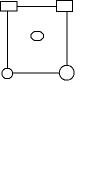
\includegraphics{week0_example}
\caption{An example for including graphics}
\label{MPS:fig:graphics}
\end{center}
\end{figure}

\subsection{References and bibligoraphy}

You should use BibTeX for references. Whenever you want to cite a
paper you should use the command \verb!\cite{key}! where
\verb!key! consists of last name of the first author, the first
two letters of all other authors, and the last two digits of the
publication year. For example, to cite a 1981 paper by Frankl and
Wilson you should use \verb!\cite{FranklWi81}!. The result is
\cite{FranklWi81}

You should then find a BibTeX entry for the paper and place it in
your \texttt{week$x$.bib} file (where $x$ is the week number).
Don't forget to change the key to the formal prescribed above. For
example, the BibTeX entry for the Frankl and Wilson paper
\cite{FranklWi81} is:

\begin{verbatim}
@article {FranklWi81,
    AUTHOR = {Frankl, P. and Wilson, R. M.},
     TITLE = {Intersection theorems with geometric consequences},
   JOURNAL = {Combinatorica},
  FJOURNAL = {Combinatorica. An International Journal of the J\'{a}nos Bolyai
              Mathematical Society},
    VOLUME = {1},
      YEAR = {1981},
    NUMBER = {4},
     PAGES = {357--368},
      ISSN = {0209-9683},
     CODEN = {COMBDI},
   MRCLASS = {05C35 (05A17 05A20 05C15)},
  MRNUMBER = {84g:05085},
MRREVIEWER = {E. C. Milner}, }
\end{verbatim}

Once you do this, and run \LaTeX\ on the \texttt{.tex} file,
BibTeX on the \texttt{.bib} file, and then again LaTeX twice on
the \texttt{.tex} file, the bibliography will be added
automatically.

\paragraph{Finding BibTeX entries.} you can find BibTeX entries
for papers on the web. A very resource is the following:

\begin{itemize}

\item zbMATH Open:
\url{https://zbmath.org/}
\end{itemize}



\section{Useful macros that are predefined for you}

The template\footnote{Actually, these are defined in the file
\texttt{template.sty} which you can view but SHOULD NOT MODIFY!.}
already contains the following \LaTeX\ commands and environments.
If you want to define additional commands, you need to prefix them
with the initials of your name.

\subsection{Math Symbols (partial list)}
\newcommand{\seprt}{&}

\begin{tabular}{llll}
\verb!\eqdef! : $\eqdef$   \\
\verb!\N! : $\N$ \seprt \verb!\R! :
$\R$ \seprt \verb!\Z! : $\Z$ \\
\verb!\C! : $\C$ \seprt \verb!\F! : $\F$ \\
\verb!\getsr! : $\getsr$ \seprt \verb!\st! : $\st$ \seprt
\noindent \verb!\Ex! : $\Ex$ \\
\verb!\e! : $\e$ \\
\verb!\To! : $\To$ \\
\verb!\ceil{x}! : $\ceil{x}$ \seprt \verb!\floor{x}! : $\floor{x}$
\seprt \verb!\angles{x,y,z}! : $\angles{x,y,z}$ \\
\verb!\norm{x}{\infty}! : $\norm{x}{\infty}$ \seprt
\verb!\normone{x}! : $\normone{x}$ \seprt \verb!\normtwo{x}! :
$\normtwo{x}$ \\
\verb!\dprod{x}{y}! : $\dprod{x}{y}$  \seprt \verb!\bits! : $\bits$ \\
\verb!\poly! : $\poly$ \seprt \verb!\polylog! : $\polylog$ \\
\verb!\GF! : $\GF$ \seprt \verb!\charfun{S}! : $\charfun{S}$
\end{tabular}

%\newcommand{\poly}{{\rm poly}}
%\newcommand{\polylog}{{\rm polylog}}
%\newcommand{\GF}{\mathrm{GF}}
%\newcommand{\charfun}[1]{{\bf{1}}_{#1}}


In addition, all the AMS\LaTeX\ macros are available. Particularly
useful macros are \verb!\binom{}{}! for the binomial coefficient
(e.g. $\binom{n}{k}$), \verb!\pmod{}! for modular equations (e.g.,
$2=9 \pmod{7}$),  \verb!\tfrac{}{}! for fractions that take less
vertical space (e.g. $\tfrac{3}{4}$), and \verb!\vec{}! for
vectors (e.g., $\vec{v}$). You can find more information about
AMS\LaTeX\ in the tutorials mentioned above and in the AMS\LaTeX
user guide. If you are writing fractions inline then always use \verb!\dfrac{}{}!.

\subsection{Environments}

List of environments:

\begin{itemize}

\item  Theorems etc.: \textbf{theorem} , \textbf{claim} , \textbf{subclaim} (for a claim
inside a proof of a theorem) , \textbf{lemma} , \textbf{corollary}
, \textbf{conjecture} , \textbf{observation}.

\item Definitions etc.: \textbf{definition} ,
\textbf{construction}, \textbf{example} , \textbf{remark}

\item Exercises etc.: \textbf{exercise} and \textbf{answer}
\end{itemize}

Some examples:

\begin{definition} \label{MPS:def:bal} A function $f:\bits^n \To
\bits$ is \emph{balanced} if
\[
\Pr_{x \getsr \bits^n}[  f(x)= 1 ] = \frac{1}{2}.
\]
\end{definition}

\begin{theorem} \label{MPS:thm:prod} For every $\alpha \in \bits^n$,
let $f_{\alpha}:\bits^n \To \bits$ denote the following function
$f_{\alpha}(x) = \dprod{x}{\alpha}$. Then, $f_{\alpha}$ is
balanced.
\end{theorem}

\begin{algorithm}[Computing a square root] \label{MPS:alg:sqroot}
\textbf{Input:} $n \in \N$

\begin{enumerate}

\item Let $l \leftarrow 0$, $h \leftarrow n$.

\item Do the following while $h>l$:

\begin{enumerate}
\item  Let $m \leftarrow
\left\lfloor\dfrac{l+h}{2}\right\rfloor$.

\item If $m^2 < n$ then let $l \leftarrow m$. Otherwise, let $h
\leftarrow m$.

\end{enumerate}

\item Output $m$.
\end{enumerate}

\end{algorithm}

Which were produced by
\begin{verbatim}
\begin{definition} \label{MPS:def:bal} A function $f:\bits^n \To
\bits$ is \emph{balanced} if
\[
\Pr_{x \getsr \bits^n}[  f(x)= 1 ] = \frac{1}{2}
\]
\end{definition}

\begin{theorem} \label{MPS:thm:prod} For every $\alpha \in \bits^n$,
let $f_{\alpha}:\bits^n \To \bits$ denote the following function
$f_{\alpha}(x) = \dprod{x}{\alpha}$. Then, $f_{\alpha}$ is
balanced.
\end{theorem}
\end{verbatim}

\begin{verbatim}
\begin{algorithm}[Computing a square root] \label{MPS:alg:sqroot}
\textbf{Input:} $n \in \N$

\begin{enumerate}

\item Let $l \leftarrow 0$, $h \leftarrow n$.

\item Do the following while $h>l$:

\begin{enumerate}
\item  Let $m \leftarrow
\left\lfloor\dfrac{l+h}{2}\right\rfloor$.

\item If $m^2 < n$ then let $l \leftarrow m$. Otherwise, let $h
\leftarrow m$.

\end{enumerate}

\item Output $m$.
\end{enumerate}

\end{algorithm}
\end{verbatim}

% END BODY of document
%%%%%%%%%%%%%%%%%%%%%%%%%%%%%%%%%%%%%%%%%%%%%%%%%%%%%%%%%%%%%%%%%%%%%%%%%
\ENDDOC

%%%%%%%%%%%%%%%%%%%%%%%%%%%%%%%%%%%%%%%%%%%%%%%%%%%%%%%%%%%%%%%%%%%%%%%%%%%%%%%%%%%%%%%%%%%%%%%%%%%%%%%%%%%%%%%%%%%%%%%%%%%%%%%%


